 	%%%%%%%%%%%%%%%%%%%%%%%%%%%%%%%%%%%%%%%%%
% Stylish Article
% LaTeX Template
% Version 2.2 (2020-10-22)
%
% This template has been downloaded from:
% http://www.LaTeXTemplates.com
%
% Original author:
% Mathias Legrand (legrand.mathias@gmail.com) 
% With extensive modifications by:
% Vel (vel@latextemplates.com)
%
% License:
% CC BY-NC-SA 3.0 (http://creativecommons.org/licenses/by-nc-sa/3.0/)
%
%%%%%%%%%%%%%%%%%%%%%%%%%%%%%%%%%%%%%%%%%

%----------------------------------------------------------------------------------------
%	PACKAGES AND OTHER DOCUMENT CONFIGURATIONS
%----------------------------------------------------------------------------------------

\documentclass[fleqn,10pt]{SelfArx} % Document font size and equations flushed left
\usepackage{listings}
\lstnewenvironment{captioned_code}[1][]{%
	\lstset{
		basicstyle=\ttfamily,
		frame=tb,
		#1
	}%
}{}

\usepackage[english]{babel} % Specify a different language here - english by default
%\usepackage[
%backend=biber,
%style=alphabetic,
%]{biblatex}
%\bibliographystyle{ref.bib}
\usepackage{lipsum} % Required to insert dummy text. To be removed otherwise

%----------------------------------------------------------------------------------------
%	COLUMNS
%----------------------------------------------------------------------------------------

\setlength{\columnsep}{0.55cm} % Distance between the two columns of text
\setlength{\fboxrule}{0.75pt} % Width of the border around the abstract

%----------------------------------------------------------------------------------------
%	COLORS
%----------------------------------------------------------------------------------------

\definecolor{color1}{RGB}{244,130,115} % Color of the article title and sections
\definecolor{color2}{RGB}{200,60,10} % Color of the boxes behind the abstract and headings
\definecolor{color3}{RGB}{120, 140, 190} % Color of links
%----------------------------------------------------------------------------------------
%	HYPERLINKS
%----------------------------------------------------------------------------------------

\usepackage{hyperref} % Required for hyperlinks

\hypersetup{
	hidelinks,
	colorlinks,
	breaklinks=true,
	urlcolor=color3,
	citecolor=color1,
	linkcolor=color1,
	bookmarksopen=false,
	pdftitle={Title},
	pdfauthor={Author},
}
\newcommand{\link}[2]{
  \href{#2}{\bf[#1]}
}
%----------------------------------------------------------------------------------------
%	ARTICLE INFORMATION
%----------------------------------------------------------------------------------------

\JournalInfo{Laboratory Report for the Algorithms and Data Structures Laboratory Class} % Journal information
\Archive{of the University of Florence} % Additional notes (e.g. copyright, DOI, review/research article)

\PaperTitle{A Comparative Benchmark of Multiset Binary Search Tree Variants: Regular, Alternating and List-Grouped} % Article title

\Authors{Besnik Nuro} % Authors
%\affiliation{\textsuperscript{1}\textit{Department of Biology, University of Examples, London, United Kingdom}} % Author affiliation
%\affiliation{\textsuperscript{2}\textit{Department of Chemistry, University of Examples, London, United Kingdom}} % Author affiliation
%\affiliation{*\textbf{Corresponding author}: john@smith.com} % Corresponding author

\Keywords{Binary Search Tree -- Multiset -- Benchmark} % Keywords - if you don't want any simply remove all the text between the curly brackets
\newcommand{\keywordname}{Keywords} % Defines the keywords heading name

%----------------------------------------------------------------------------------------
%	ABSTRACT
%----------------------------------------------------------------------------------------

\Abstract{The Binary Search Tree is a fundamental data structure used for its logarithmic ordered search time complexity. While traditionally not meant to store duplicate keys, certain applications, for example ones involving colliding hashed keys or word frequency counters may warrant handling of duplicates in a certain manner. In this laboratory report three multiset implementations are put against each-other to measure performance when duplicates are used: Regular Insertion BST, Alternating Insertion BST and a multiset BST with a duplicate collection.}

%----------------------------------------------------------------------------------------

\begin{document}

\maketitle % Output the title and abstract box

\tableofcontents % Output the contents section

\thispagestyle{empty} % Removes page numbering from the first page

%----------------------------------------------------------------------------------------
%	ARTICLE CONTENTS
%----------------------------------------------------------------------------------------

\section*{A bit of theory} % The \section*{} command stops section numbering

\addcontentsline{toc}{section}{A bit of theory} % Adds this section to the table of contents
Multiset collections are sets in which duplicates are allowed. A Multiset Binary Search Tree would be a Binary Search Tree (BST) with the ability to insert and manage duplicates.

A regular implementation of a BST allows for duplicates but they are made inaccessible unless deletions are used.

An Alternating BST would be a BST in which insertion of duplicates is alternated between the left and right nodes.

For example, three equivalent keys inserted in succession degenerate to a linked list in a regular BST but in an Alternating BST they are equivalent to the first insertion being a parent with the other two nodes as left and right siblings. In fact it can be trivially proven that for a succession of $n$ equivalent key insertions, a balanced subtree of duplicates forms.

An untitled Multiset BST implementation, here called List-Grouped BST, stores duplicates in a list (optionally linked) pointed to by the first equivalent node inserted. This implementation has the advantage of easy retrieval of the values and shorter heights which imply shorter search times. If a succession of $n$ equivalent keys increases height by $n$ in a regular BST implementation, $\log_2(n)$ in an Alternating BST, in a List-Grouped BST the height is increased by one level and the rest of the duplicates are stored in multiset collections pointed to by the nodes. This implementation is also more space-efficient if keys are not stored in node containers inside the collection.
%\footnote{And some mathematics $\cos\pi=-1$ and $\alpha$ in the text.}.

%------------------------------------------------

\section{Basis and Experiments}

%\begin{figure*}[ht]\centering % Using \begin{figure*} makes the figure take up the entire width of the page
%	\includegraphics[width=\linewidth]{architecture}
%	\caption{Producer-Broker Architecture}
%	\label{fig:architecture}
%\end{figure*}

To have an idea of why the data structures exist and how experiments were formulated, a description of the problem is in order.

\subsection{The need for multiple keys}
Multiple key handling is required when BSTs are used to implement more advanced data structures.  
\subsubsection{Priority Queues}
Priority Queues are data structures often used for task scheduling in operating systems. More generally, they can be used in any application where a data structure of elements ordered by priority is needed. For example, a CPU with distinct performance and efficiency cores can make use of a task scheduler which uses a Multiset BST-based Priority Queue to retrieve tasks with lower (but sometimes equal) priority for the efficiency cores. This is preferable to a heap implementation which favors highest priority retrieval.

\subsubsection{Maps}
Maps are sometimes implemented as self-balancing BSTs. This implementation is simpler compared to using a hash table. \verb|std::map| uses a self-balancing BST in its implementation. The motive for handling duplicate keys arises when hashed keys can collide with each-other.

\subsubsection{Order Statistics}
Order-Statistics Binary Search Trees (OS-BST) are used for order statistics to efficiently find elements by their rank and perform range queries. A multiset implementation is needed since there can be elements with the same key. Examples are text analyzers and analytics/statistics in different fields.

\subsection{Why a regular BST is not enough}
The advantage Binary Search Trees offer is that they have fast ($O(\log_2(n))$) query times, as long as they are balanced. In case of left-skewed subtrees (one produced by successive duplicate insertion), the query time within that subtree is $O(n)$. This is because it is no different from a linked list search. 

The search time is proportional to the height of a given tree, so the more balanced a Binary Search Tree, the faster the query time. By accounting for duplicates in the implementation of a Binary Search Tree, we can reduce this height via alternate insertion or collection insertion in accordance with the application intended for the data structure.

\subsection{Implementations}
We consider the three implementations mentioned in the introduction.
\subsubsection{Regular BST with left-biased insertion}
A regular BST node is a structure containing:
\begin{itemize}
 \item a parent node reference;
 \item two (\texttt{left\_node} and \texttt{right\_node}) references to sibling nodes;
 \item a key which is for sorting values;
 \item a value contained or pointer to it;
 \item a root reference;
\end{itemize}
In these implementations, for the sake of simplicity, \texttt{value} refers to both the key and value contained. There is no reason why these implementations wouldn't work for different key and value attributes.
\begin{captioned_code}[title={Python code for BST node structure}]
class BinarySearchTree():
    def __init__(self, value):
        self.parent = None
        self.left_node = None
        self.right_node = None
        self.value = value
        self.root = self
\end{captioned_code}
Initializing a tree as \texttt{BinarySearchTree(n)} creates a root node containing n as its value. It and every successive node points to itself when queried for the root node. This way subtrees are conceptually implemented.

A \texttt{print(node)} will print the subtree with \texttt{node} as its parent key. This is because \texttt{\_\_str\_\_} returns the string representation of a class which the print function uses. By overriding \texttt{\_\_str\_\_} we can give a tree an presentable visual representation.
\begin{captioned_code}[title={For the documentation of the code, check Appendix A.}]
def __str__(self):
    return (self
    ._BinarySearchTree__tree_walk_helper())
\end{captioned_code}
Insertion in this case would be as the left node of the equivalent parent. When queried for a key, the tree returns the first node matching the queried key. That means only one node reference is returned for any amount of equivalent keys and the keys not returned are inaccessible unless the any nodes coming before them in order are deleted.

\subsubsection{BST with alternating insertions}
The implementation of this structure is the same as for the regular BST, with the exception of an additional attribute \texttt{preferLeft} and a few more lines in the logic of the \texttt{insert} method. For each successful insertion, the value of \texttt{preferLeft} is alternated between \texttt{False} and \texttt{True}.

\subsubsection{BST with collection for duplicates}
This implementation differs from the regular and the alternating one in that each node points to an collection for duplicates. Insertion here does not inser
t in the tree if there are duplicates, but in an appropriate collection instead. In our implementation we have used a list, but a deque could be used instead for fast insertions and deletions.

Querying for a key contained in the tree returns the node and a flag which asserts whether there are dupes for that key. \texttt{get\_duplicates} returns a reference to the collection of duplicates.

\subsubsection{Expectations}
We can expect a regular BST's height to increase linearly for each successive duplicate insertion. For low collision rates this should not be a problem. 

An alternating BST's height should increase logarithmically for each successive duplicate insertion. For example, for 5 equivalent insertions, the height should increase by 3 and for 100 it should increase by 7. This would be the same rate of increase as a regular BST with random insertions.

A list-grouped BST's height should increase by one node for any succession of equivalent insertions. This means that for $n$ equivalent insertions, the height increases by one and the list of duplicates pointed to by the node increases in size by $n-1$.

\subsubsection{Experiments}
Different test cases were devised in order to confirm or deny the expectations. There is a baseline test case for randomly inserted keys. This will be used to compare against. Another reference would be the upper bound of the worst case (all duplicate insertions), which will not be graphed and has already been mentioned in the introduction and problem formulation.

There are two test cases intended to mimic low collision rates of samples and hashed keys:
\begin{itemize}
	\item $0.01\%$ collision rate
	\item $0.05\%$ collision rate
\end{itemize}

Two more cases intended for moderate collision rates of samples:
\begin{itemize}
	\item $0.1\%$ collision rate
	\item $0.5\%$ collision rate
\end{itemize}

Three cases are intended for high collision rates of samples:
\begin{itemize}
	\item $1\%$ collision rate
	\item $5\%$ collision rate
	\item $10\%$ collision rate
\end{itemize}

The data structures will be tested for the insertion of 1000, 5000, 10000 elements with the appropriate collision rates for each test case. Collision rate is $\frac{1}{\texttt{max\_value}}$.

\begin{captioned_code}[title=Test Case for 0.1\% Collision Rate]
    max_value = 999
    size = 10000
    root_value = max_value//2
    
    regular = \
    BinarySearchTree(root_value)
    alternating = \
    AlternatingBinarySearchTree(root_value)
    listgrouped = \
    ListGroupedBinarySearchTree(root_value)

    for i in \
    	SyntheticData. \
    	generate_integer_list(size,
    		max_value):
        regular.insert(i)
        alternating.insert(i)
        listgrouped.insert(i)
\end{captioned_code}

The height for each tree is recorded after the insertions and exported to a file. This way tests can be run in batch.
\begin{captioned_code}[]
    output = \
    str(regular.get_height()) + " " + \
    str(alternating.get_height()) \
    + " " + \
    str(listgrouped.get_height())
    
    Export.export_values_to_file(output)
\end{captioned_code}

The exported data is listed in columns, each column containing values for a BST's test case results.
\begin{captioned_code}[]
# cat data/export
18 13 6
20 11 5
19 10 5

\end{captioned_code}
A shell loop was used to run many cases sequentially so that a mean value could be extracted. For this report, a hundred runs were made.
\begin{captioned_code}[]
for i in {1..n}
	do python bst/main.py
done 
\end{captioned_code}
\iffalse
Reference to figure \ref{fig:results}.
\begin{figure}[ht]\centering
	\includegraphics[width=\linewidth]{results}
	\caption{In-text Picture}
	\label{fig:results}
\end{figure}

\fi

%------------------------------------------------

\section{Results}
	The data was generated via a few bash scripts using awk for processing of the data and gnuplot for plot generation. The data were approximated with bezier curves.

\subsection{Low Collision Rates}
For low collision rates, the regular and the alternating variants of the BST perform similarly and there is a slight gain of performance only for list-grouped BSTs.

\begin{figure}[ht]\centering
	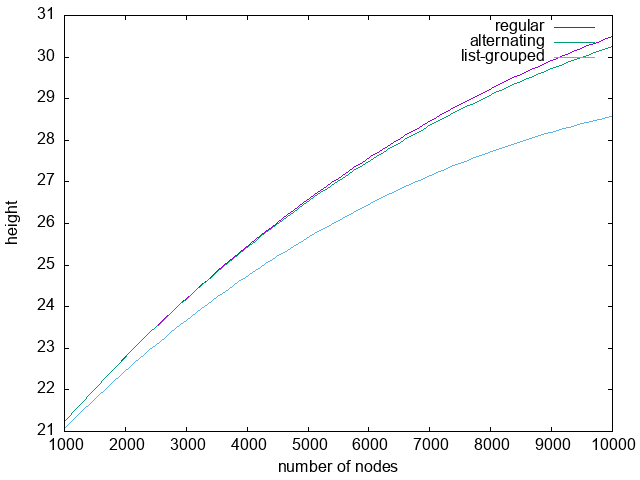
\includegraphics[width=\linewidth]{Figures/0.01_plot.png}
	\caption{0.01\% Collision Rate Plot}
	\label{fig:0.01_plot}
\end{figure}


\subsubsection{0.01\% Collision Rate}

The regular and alternating BSTs perform almost identically, with the alternating BST height being slightly lower. The list-grouped version has a lower height, but not by much.

\subsubsection{0.05\% Collision Rate}

Results are similar to the 0.01\% collision rate case.
\begin{figure}[ht]
	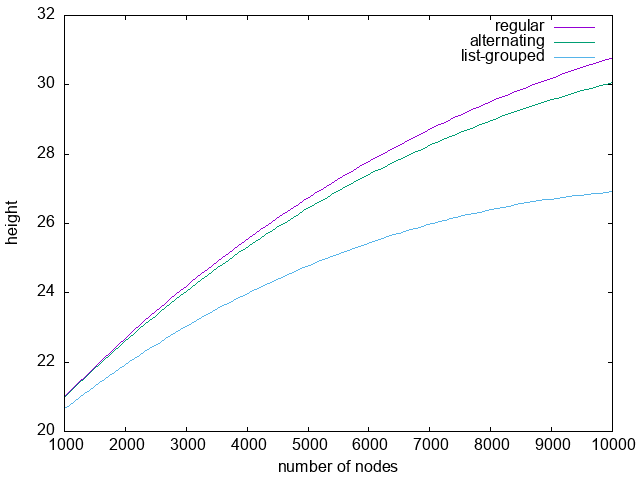
\includegraphics[width=\linewidth]{Figures/0.05_plot.png}
	\caption{0.05\% Collision Rate Plot}
	\label{fig:0.05_plot}
\end{figure}

\subsection{Moderate Collision Rates}
In moderate collision rate test cases, alternating BSTs and list-grouped BSTs start to show their resistance to height scaling with respect to duplicates.
\subsubsection{0.1\% Collision Rate}
Here we see the first considerable difference between the three BST variants. While the regular BST scales almost linearly, the alternating BST performs much better, still retaining the logarithmic scaling of the height. List-grouped BST has an almost linear height scaling. 

\begin{figure}[ht]\centering
	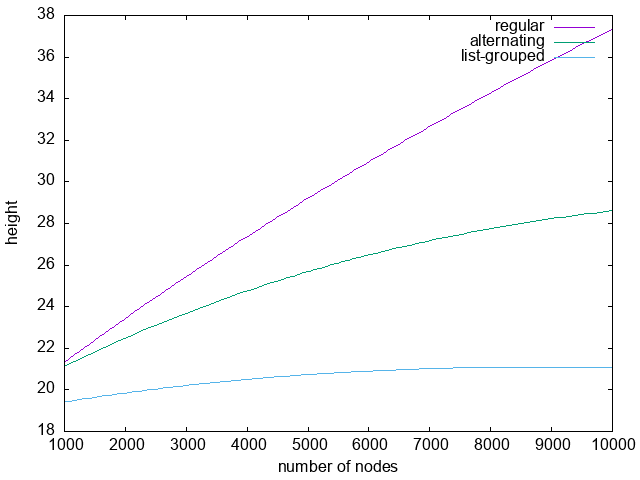
\includegraphics[width=\linewidth]{Figures/0.1_plot.png}
	\caption{0.1\% Collision Rate Plot}
	\label{fig:0.1_plot}
\end{figure}

\subsubsection{0.5\% Collision Rate}
In the 0.5\% test case, the difference is even more pronounces. While the regular implementation continues to scale linearly, the other two variants fare better: there are enough repetitions for these two BST implementations to make use of their properties. Interestingly, the height of the list-grouped BST remains constant on average with respect to the lower bound of 1000 elements. This may imply that for this collision rate any application that foresees a structure with more elements than this lower bound, the use of the list-grouped implementation is the most beneficial one.

\begin{figure}[ht]\centering
	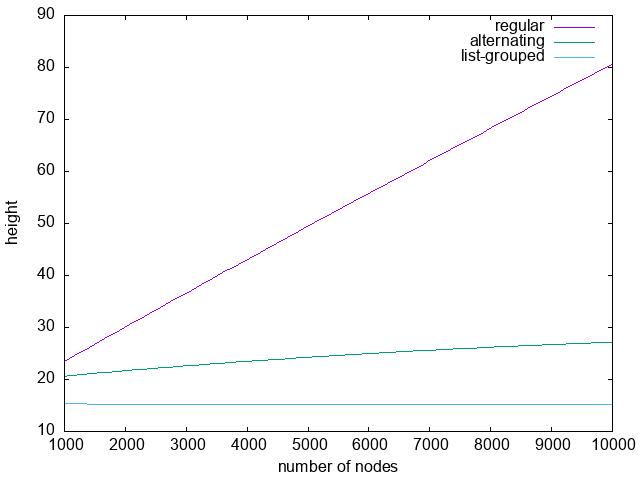
\includegraphics[width=\linewidth]{Figures/0.5_plot.png}
	\caption{0.5\% Collision Rate Plot}
	\label{fig:0.5_plot}
\end{figure}

\subsection{High Collision Rates}

\begin{figure}[ht]\centering
	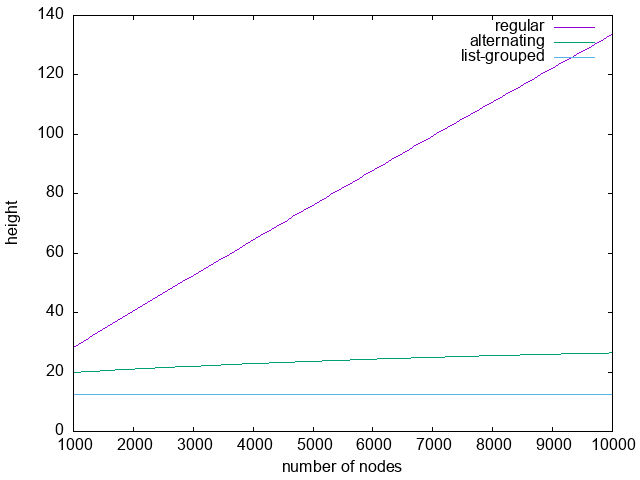
\includegraphics[width=\linewidth]{Figures/1_plot.png}
	\caption{1\% Collision Rate Plot}
	\label{fig:1_plot}
\end{figure}

The common denominator for this class of test cases is that the regular implementation of the Binary Search Tree maintains a linear scaling of its height, whereas the alternating and list-grouped BSTs show a constant or almost constant height on average. In fact:
\begin{itemize}
	\item for a 1\% collision rate, the height of list-grouped had an average of 12.6 and did not surpass 17;
	\item for a 1\% collision rate, the height of alternating had an average of 26.4 and did not surpass 31;
	\item for a 5\% collision rate, the height of list-grouped had an average of 7.2 and did not surpass 9;
	\item for a 5\% collision rate, the height of alternating had an average of 24.8 and did not surpass 31;
	\item for a 10\% collision rate, the height of list-grouped had an average of 4.9 and did not surpass 6;
	\item for a 10\% collision rate, the height of alternating had an average of 24.2 and did not surpass 27;
\end{itemize}

\begin{figure}[ht]
	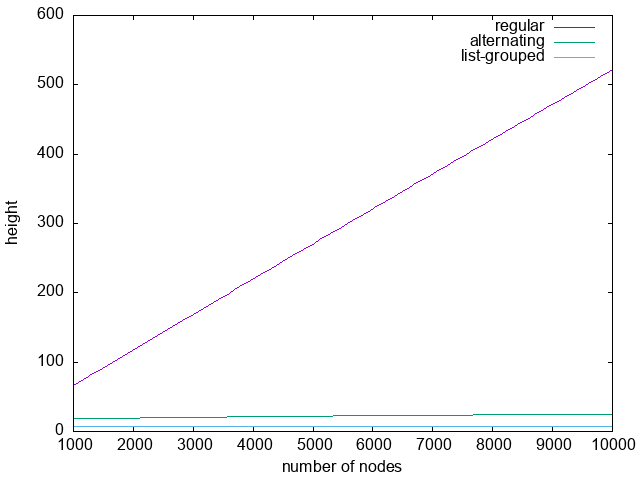
\includegraphics[width=\linewidth]{Figures/5_plot.png}
	\caption{5\% Collision Rate Plot}
	\label{fig:5_plot}
\end{figure}
%\phantomsection

\begin{figure}[ht]
	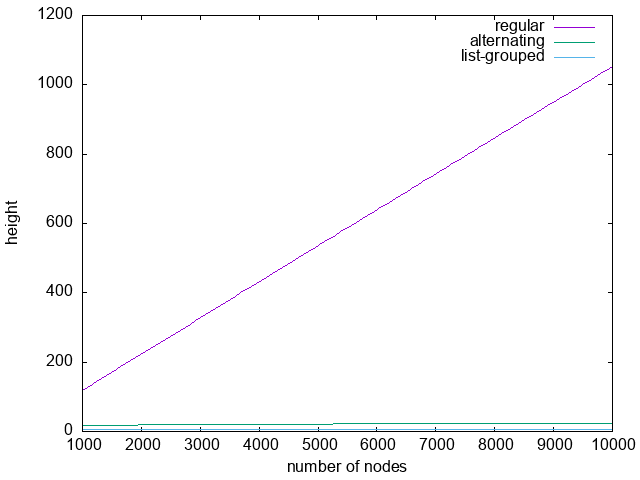
\includegraphics[width=\linewidth]{Figures/10_plot.png}
	\caption{10\% Collision Rate Plot}
	\label{fig:10_plot}
\end{figure}

\section{Analysis and Interpretation}
As hinted before, low collision rate test cases were meant to mimic applications where keys rarely collide. Hashed keys are one such example. Typically they have very low collision rates, but we can already see that in the 0.01\% collision rate test case the regular and alternating BSTs perform almost identically, leading us to believe that for lower rates of collision this should be true as well. We can say the alternating BST implementation does not have any significant benefits in these conditions with respect to the regular implementation. However, the list-grouped BST scales a bit better in the 0.05\% collision rate. With this in mind we can see that list-grouped BSTs may be worth it where performance is more of an issue and we don't have access to better alternatives.

For moderate collision rates the trade-offs become more apparent:
\begin{itemize}
	\item height of the regular BST starts to increase linearly with respect to the previous test class. This means that for uniformly-distributed ranges of keys with collision rates equal or higher to 0.1 percent, the regular BST start to throttle in performance.
	\item height of the list-grouped BST starts to look more like a constant line. We can take this to mean that from this point on the collection BST implementation fairs better for searches than its competitors.
	\item the alternating BST is somewhere in the between: whether of not to use it remains to the be decided by further circumstances. For example, in a application where performance is critical this variant wouldn't be useful, whereas in another where we want moderate performance for searches it can be decently performant.
\end{itemize}

High collision rate test cases were meant to roughly simulate instances in which repetitions are common or probable. One such case could be a frequency analyzer for a text or for a corpus of population data with respect to certain attributes such as name, surname or region of provenance. Regardless of the actual application, this class of tests shows that even an alternating Binary Search Tree can be useful, almost as much as a list-grouped Binary Search Tree. Regular implementations, on the other hand, scale with a complexity between linear and logarithmic. Locally, between the 1000 and 10000 elements it behaves almost linearly. Even insertion times during tests were increased noticeably for this class of collision rates with respect to the other test cases.

\clearpage

\section{Appendix A: Code Documentation}

\begin{figure}[ht]
	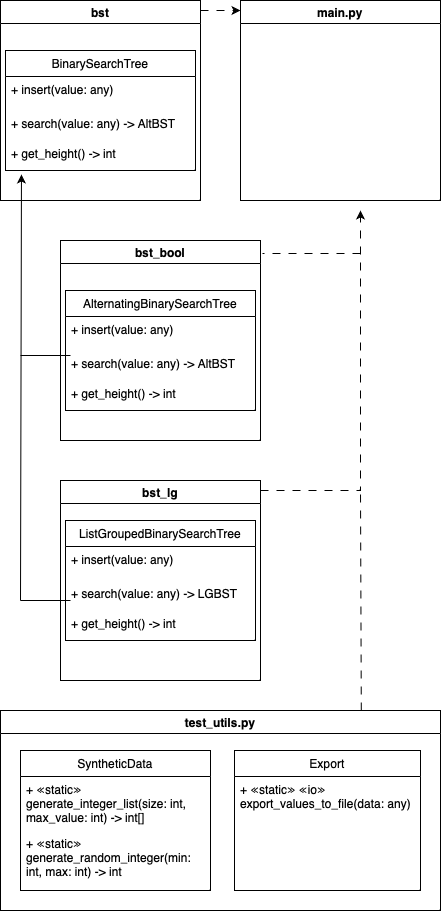
\includegraphics[width=\linewidth]{interactions}
	\caption{Module and Class Interaction Diagram}
	\label{fig:interactions}
\end{figure}

\subsection*{BinarySearchTree}
\subsubsection*{\_\_init\_\_(self, value)}
Initializes a tree with the root node as itself, contained value/key with the given value, null pointers to siblings nodes and parent node. 
\subsubsection*{\_\_str\_\_(self)}
Override of the \texttt{\_\_str\_\_} method, returns a visual string representation via a tree walk.
\subsubsection*{\_\_tree\_walk\_helper(self)}
Helper wrapper for the \texttt{\_\_tree\_walk} method.
\subsubsection*{\_\_tree\_walk(self, buffer, vbranch)}
Calls itself recursively to construct a visual tree representation stored in the buffer via an in-order tree traversal. Returns a string representation of the tree for visual debugging.
\subsubsection*{insert(self, new\_value)}
Performs a textbook Binary Search Tree insertion. Left-biased for duplicates. Returns a reference to the new node.
\subsubsection*{search(self, value)}
Performs a recursive binary search for a given value on the tree. Returns a reference to the first equivalent node if found, else returns \texttt{None}.
\subsubsection*{get\_height(self)}
Returns the height of the tree.

\subsection*{AlternatingBinarySearchTree}
\subsubsection*{\_\_init\_\_(self, value)}
Initializes a tree with the root node as itself, contained value/key with the given value, null pointers to siblings nodes and parent node. Initializes \texttt{preferLeft} to \texttt{True}.
\subsubsection*{\_\_str\_\_(self)}
Override of the \texttt{\_\_str\_\_} method, returns a visual string representation via a tree walk.
\subsubsection*{\_\_tree\_walk\_helper(self)}
Helper wrapper for the \texttt{\_\_tree\_walk} method.
\subsubsection*{\_\_tree\_walk(self, buffer, vbranch)}
Calls itself recursively to construct a visual tree representation stored in the buffer via an in-order tree traversal. Returns a string representation of the tree for visual debugging.
\subsubsection*{insert(self, new\_value)}
Performs a Binary Search Tree insertion. Duplicate insertion is alternated by checking \texttt{preferLeft}, toggling it and inserting accordingly. Returns a reference to the new node.
\subsubsection*{search(self, value)}
Performs a recursive binary search for a given value on the tree. Returns a reference to the first equivalent node if found, else returns \texttt{None}.
\subsubsection*{get\_height(self)}
Returns the height of the tree.

\subsection*{ListGroupedBinarySearchTree}
\subsubsection*{\_\_init\_\_(self, value)}
Initializes a tree with the root node as itself, contained value/key with the given value, null pointers to siblings nodes and parent node, and a null pointer for a list of duplicates to be initialized upon duplicate insertion.
\subsubsection*{\_\_str\_\_(self)}
Override of the \texttt{\_\_str\_\_} method, returns a visual string representation via a tree walk.
\subsubsection*{\_\_tree\_walk\_helper(self)}
Helper wrapper for the \texttt{\_\_tree\_walk} method.
\subsubsection*{\_\_tree\_walk(self, buffer, vbranch)}
Calls itself recursively to construct a visual tree representation stored in the buffer via an in-order tree traversal. Returns a string representation of the tree for visual debugging.
\subsubsection*{insert(self, new\_value)}
Performs a Binary Search Tree insertion. When the first duplicate for a key is inserted, it initializes the pointer to the list. Otherwise, it puts the duplicate inside the list. Returns a reference to the new node.
\subsubsection*{search(self, value)}
Performs a recursive binary search for a given value on the tree. Returns a reference to the first equivalent node if found, otherwise \texttt{None}. Also returns a flag indicating whether there are duplicates as the second positional return value.
\subsubsection*{get\_height(self)}
Returns the height of the tree.
\subsubsection*{get\_duplicates(self)}
Returns a reference to the list of duplicates for its node.

\subsection*{SyntheticData}
\subsubsection*{generate\_integer\_list(size, max\_value)}
Returns a list of length equal to \texttt{size} and with values ranging from 0 to \texttt{max\_value} inclusive.
\subsubsection*{generate\_random\_integer(min, max)}
Returns an integer between \texttt{min} and \texttt{max} inclusive. Originally used for debugging.

\subsection*{Export}
\subsubsection*{export\_values\_to\_file(data)}
Creates a file called \texttt{export} inside the \texttt{data} directory and writes the string representation of the passed argument to it.


\section{Appendix B: Explanations about choices}
\subsection*{Why isn't there a Node class?}
	Nodes and BSTs are represented as the same structure. The reason for this is that programming the logic for two separate structures increased the complexity of the code without adding meaningful improvements. However, it is possible for the variants to extend a class representing a vertex or node without affecting any of the functionality provided by this implementation. I didn't do this because it would not be very useful to have a \texttt{Node} class with only a string representation method and a value reference inside, especially when the inheriting classes would contain them anyway.

\subsection*{Why is the measure the height of the trees and not the time required for insertions and searches?}
	Since the upper bound for time of an insertion or search takes is linked to the height of the tree, measuring height offers us a proxy and a way to measure expected performance without actually timing results. This means that regardless of the machine in which tests are run, the expected performance should be proportional to height. Indeed, a higher tree took longer to populate on average when I ran the tests.
	
\subsection*{How were the data and plots generated?}
Each test case was manually ran a hundred times for each population of 1000, 5000 and 10000 nodes. Height was measured and written in columns in a text file. The first column represents a regular BST, the second an alternating BST and the third a list-grouped BST. In this manner a $100 \times 3$ matrix was created. The columns were reduced to averages via a \texttt{apply\_avg.sh}, a shell script using awk to average the columns. These averages were then plotted using \texttt{gnuplot} with 1000, 5000 and 10000 insertions as ordinates.

\subsection*{Where can I find the data used for this report?}
The \texttt{data} directory contains all data used to generate the plots, while \texttt{utils} contains scripts and intermediary data relevant to the original data.

%------------------------------------------------
%\section*{References} % The \section*{} command stops section numbering

%\addcontentsline{toc}{section}{References} % Adds this section to the table of contents
%\printbibliography[title={References}]

%----------------------------------------------------------------------------------------

\end{document}